\section{引言}
在大数据时代,人们越来越依赖数据分析进行决策~\cite{albright2020business}。例如,当一家超市想要通过明智的库存管理来优化其利润时,它需要考虑各种因素,如历史销售订单、客户偏好、不同商品的利润率等。这通常需要分析来自各个方面的海量数据来做出明智的决策。

为了执行数据分析,没有自己服务器的个人通常将数据分析任务委托给云服务器~\cite{sandhu2021big}。然而,在使用云服务器进行数据分析时,人们担心这些关键数据可能被泄露~\cite{purohit2013data},因为它通常涉及个人隐私或商业机密。

为了解决数据泄露问题,越来越多的相关技术被提出。这些技术包括:安全多方计算(MPC)~\cite{lindell2020secure,patra2021aby2,dalskov2022fast}、同态加密(HE)~\cite{marcolla2022survey,lu2021pegasus,bossuat2021efficient}、联邦学习(FL)~\cite{li2021survey,bonawitz2017practical,shayan2020biscotti}、可信执行环境(TEE)~\cite{zheng2021survey,tsai2017graphene,priebe2018enclavedb}。

在这些技术中,TEE具有通用性,适用于各种通用计算场景,并提供更高的计算性能。

然而,随着涉及多个角色的数据分析场景日益复杂,现有技术无法直接应用于这些复杂场景来有效解决数据泄露问题。

在现有的数据分析场景中,只有两个角色,如图~\ref{fig:analysis_scenarios}(a)所示:租户和云服务提供商。现有技术主要专注于防止云服务提供商泄露租户数据。然而,在当今的数据分析场景中,涉及多个角色,如图~\ref{fig:analysis_scenarios}(b)所示,包括数据提供方、数据使用方、模型提供方和云服务提供商。数据必须防止被数据提供方之外的所有方泄露。除此之外,还需要保护数据分析场景中所有相关方的利益。例如,数据使用方应该获得公平有效的分析结果,而数据提供方、模型提供方和云服务提供商应该进行公平的收入分配。

因此,在处理涉及多个角色的数据分析场景时,我们需要检测数据使用方是否试图通过从计算结果中提取敏感信息来泄露数据,模型提供方是否通过恶意模型进行数据泄露,云服务提供商是否通过操纵虚拟机监控程序、操作系统、内存、磁盘等方式进行数据泄露,以及数据提供方、模型提供方和云服务提供商共同生成的计算结果是否合法。

许多相关研究被提出来解决多角色数据分析场景中面临的挑战,包括SDTE~\cite{dai2019sdte}、PrivacyGuard~\cite{xiao2020privacyguard}、SPDS~\cite{wang2020spds}、Amanuensis~\cite{hardin2022amanuensis}等。
SDTE~\cite{dai2019sdte}在数据交易行业引入了一种称为"数据处理即服务"的创新模型。利用这个模型,它通过一系列交易协议实现安全的数据交易。
PrivacyGuard~\cite{xiao2020privacyguard}利用智能合约定义数据使用策略,并利用TEE进行高效的合约执行,同时保护私有数据。
SPDS~\cite{wang2020spds}与PrivacyGuard类似,使用智能合约定义数据使用策略,并实现两阶段交付协议以确保计算结果和支付的安全发布。
Amanuensis~\cite{hardin2022amanuensis}探索了区块链技术和TEE的交集,以解决数据共享中的数据溯源、机密性和用户隐私挑战。

\begin{figure}[t]
  \centering
{
\begin{tabular}{cc}
      \subfloat[租户和云服务提供商]{
  \hspace*{-0.7cm}
        \scalebox{0.42}{
        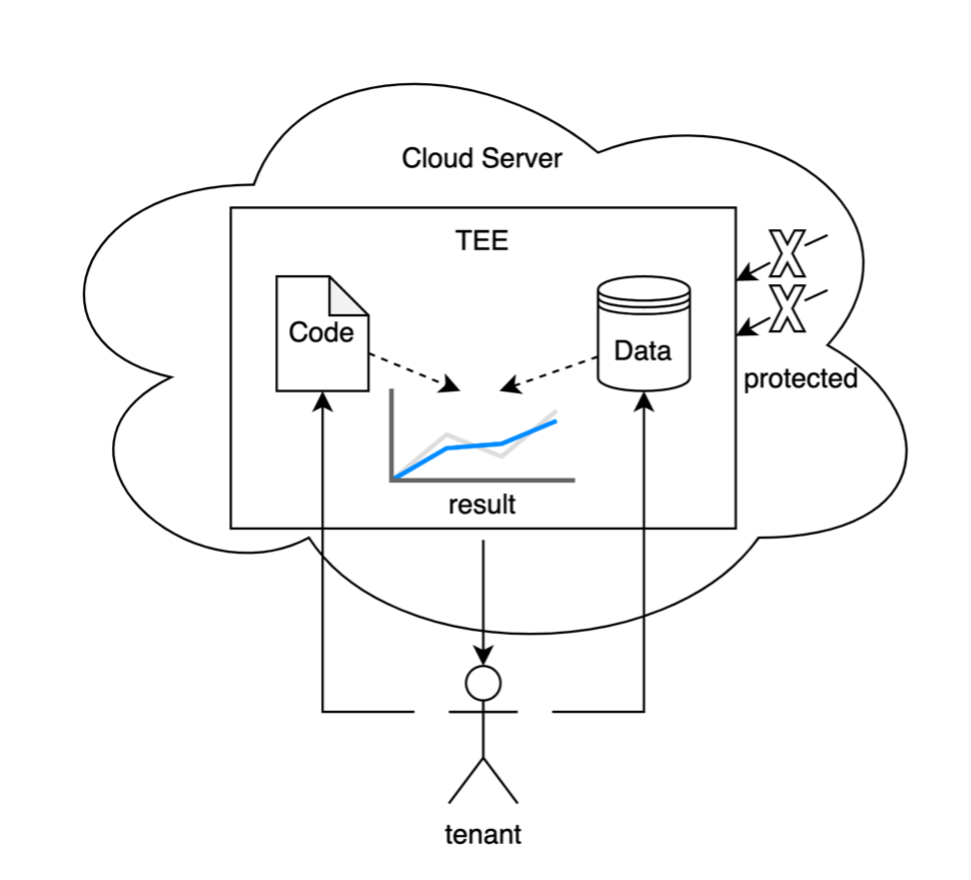
\includegraphics{images/analysis_2_roles.png}
        }
      } &
      \subfloat[多角色]{
  \hspace*{-1cm}
        \scalebox{0.42}{
        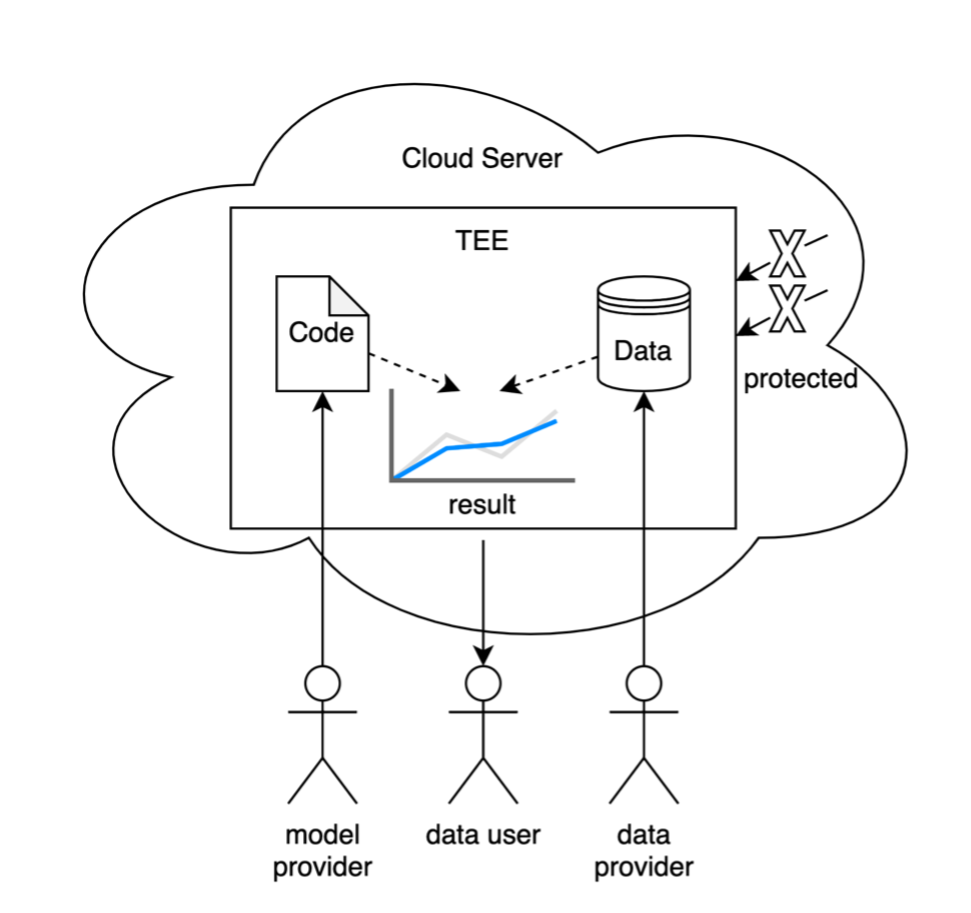
\includegraphics{images/analysis_4_roles.png}
        }
      }    \\
\end{tabular}
  }
  \caption{\small 两个角色与多角色的数据分析场景。}
  \label{fig:analysis_scenarios}
\end{figure}

然而,这些相关研究在解决这些数据分析场景时仍存在某些限制。

首先,这些相关研究工作不能保证数据分析结果中不会泄露数据。虽然这些工作引入了数据使用策略来描述谁可以以什么价格访问什么类型的数据,但数据分析程序存在恶意行为的可能性。分析程序的最终输出可能包含敏感信息的泄露。一个例子是当分析程序直接输出原始数据时,允许数据分析结果获得完整的原始数据。

一个直接的解决方案是要求分析程序公开,供数据提供方审计,确保它不包含可能导致数据泄露的代码。然而,对于模型提供方来说,他们的模型是有价值的资产,他们可能不愿意公开。另一方面,审计复杂的分析程序代表巨大的工作量,要求对每个分析任务进行审计是不可行的,因为这会显著降低数据分析的效率。

其次,现有工作无法确保计算结果的可靠性和可验证性。具体来说,当数据使用方收到计算结果时,他们无法确认这些结果确实来自通过指定模型运行指定数据,而不是简单随机生成的。此外,数据使用方缺乏任何验证这些结果正确性的方法。如果没有对计算结果的可靠性和可验证性的保证,就有可能使用欺骗性结果来误导数据使用方,损害他们的利益。

最后,在现有工作中,每个数据分析任务都需要使用远程认证来确保分析程序的一致性。然而,相关工作~\cite{chen2019opera,chen2022mage}表明,远程认证具有低效和依赖可信第三方的缺点。

以Intel软件保护扩展(SGX)增强隐私ID(EPID)为例,单次远程认证过程涉及Intel配置服务(IPS)、Intel认证服务(IAS)、Intel签名的配置enclave(PvE)、Intel签名的引用enclave(QE)和分析程序enclave之间的交互。这些交互需要通过广域网传输数据,传输的数据必须加密以确保其安全性。对于频繁的数据分析任务,这可能导致显著的性能开销。另一方面,IPS和IAS是Intel提供的集中式服务,使远程认证依赖于它们的稳定运行。

在本文中,我们提出了Fidelius,一个利用Intel SGX和区块链来增强数据分析安全性的系统,解决了前面提到的局限性。
Intel SGX确保数据分析过程的安全性和完整性,而区块链用于可信的传输、存储和验证。

为了解决计算结果中数据泄露的问题,Fidelius采用静态二进制分析方法~\cite{schulte2019gtirb}来检查模型提供的分析程序是否遵循隐私描述语言(PDL)。在这种情况下,引入的PDL将数据的计算规则描述为有限状态机(FSM),捕获从输入数据到输出数据的状态转换。任何未在PDL中描述的状态转换都被视为违反隐私规则。

为了确保计算结果的可靠性和可验证性,Fidelius提供了一个密码协议。在这个协议中,数据使用方提供一个私钥,该私钥安全地传输到分析程序的Enclave中并用于签名计算结果。由于这个私钥只能在指定的分析程序Enclave内解密,数据提供方、模型提供方和云服务提供商都无法访问。因此,如果签名的计算结果能够成功验证,就确认结果确实来自指定的分析程序并且是可验证的。

为了解决远程认证的低效和持续依赖集中式服务的问题,Fidelius结合设计的密码协议和本地认证来实现分析程序的一致性验证。Fidelius引入了密钥管理Enclave,在初始化过程中获得授权密钥。随后,在所有数据分析任务中,使用这个授权密钥执行本地认证,确保分析程序的一致性。

本文的主要贡献总结如下:
\begin{itemize}
    \item 首先,我们引入隐私描述语言(PDL)结合静态二进制分析,严格强制执行数据机密性,防止计算结果中的敏感数据泄露。
    \item 其次,我们设计了一种密码协议来确保计算结果的可靠性和可验证性。
    \item 我们集成了密码协议与本地认证机制,确保在受保护环境中执行的分析程序的完整性和正确性。
    \item 最后,我们评估了Fidelius的性能,实验结果表明它产生的开销最小,对数据分析系统的贡献不到2\%,同时超越现有解决方案30倍以上。
\end{itemize} 